\documentclass[letterpaper,10pt,titlepage,fleqn]{article}

%example of setting the fleqn parameter to the article class -- the below sets the offset from flush left (fl)
\setlength{\mathindent}{1cm}

\usepackage{graphicx}                                        
\usepackage{amssymb}                                         
\usepackage{amsmath}                                         
\usepackage{amsthm} 
\usepackage{esint}
\usepackage{nopageno}
\usepackage{booktabs}                            
\usepackage{alltt}                                           
\usepackage{float}
\usepackage{color}
\usepackage{fancyhdr}
\usepackage{url}
\usepackage{balance}
\usepackage[TABBOTCAP, tight]{subfigure}
\usepackage{enumitem}
\usepackage{pstricks, pst-node}
%the following sets the geometry of the page
\usepackage{geometry}
\geometry{textheight=9in, textwidth=6.5in}
\pagestyle{fancy}
% random comment
\newcommand{\cred}[1]{{\color{red}#1}}
\newcommand{\cblue}[1]{{\color{blue}#1}}
\usepackage{hyperref}
\usepackage{textcomp}
\usepackage{listings}
\def\name{Best CS325 Group}
%% The following metadata will show up in the PDF properties
\hypersetup{
  colorlinks = true,
  urlcolor = black,
  pdfauthor = {\name},
  pdfkeywords = {cs311 ``operating systems'' files filesystem I/O},
  pdftitle = {Pertinent Information},
  pdfsubject = {Virtual Reality Lab},
  pdfpagemode = UseNone
}

\parindent = 0.0 in
\parskip = 0.2 in
\fboxsep=5mm%padding thickness
\fboxrule=4pt%border thickness

\begin{document}
\lstset{language=Python} 

\title{Programming Assignment \#2 - CS325}

\author{
	Joshua Villwock \and
	Jaron Thatcher \and
	Ryan Phillips
}

\date{February 25, 2014}
\maketitle
%to remove page numbers, set the page style to empty







\section*{Introduction}
\hrule

In this writeup, we will both assess time complexity and prove three algorithms designed to solve the Maximum Subarray problem. 
\par

According to Wikipedia:

\par

`In computer science, the maximum subarray problem is the task of finding the contiguous subarray within a one-dimensional array of numbers (containing at least one positive number) which has the largest sum. For example, for the sequence of values $−2$, 1, $−3$, 4, $−1$, 2, 1, $−5$, 4; the contiguous subarray with the largest sum is 4, $−1$, 2, 1, with sum 6.'

\section*{Pseudocode}
\hrule
\begin{centering}

    \textbf{Brute Force:}
    \end{centering}

    \lstset{ numbers=left }

    \begin{lstlisting}%brute force pseudocode goes here

    def brute_force(x): 
      max_sum = 0
      l = len(x)
      for i in xrange(l):
        new_sum = 0
        for j in range(i,l):
          new_sum += x[j] 
          if new_sum > max_sum: max_sum = new_sum
      return max_sum

    \end{lstlisting}

    \begin{centering}
    \textbf{Divide and Conquer:}
    \end{centering}
    \begin{lstlisting}%divide and conquer pseudocode goes here

    def div_and_conq(x):
      max_sum = 0
      def inner(x,max_sum):    

        if (len(x) <= 1): # base case
          if sum(x) > max_sum:
            max_sum = sum(x)
          return max_sum

        mid = int(len(x)/2) # split into two halves
        l = x[:mid]
        r = x[mid:]

        max_sum = max(max_sum, sum(l)) # is left half max?
        max_sum = max(max_sum, sum(r)) # is right half max?

        # does max consists of suffix+prefix?
        suffix_sum = 0 
        max_suffix_sum = 0
        for i in range(mid-1,-1,-1):
          suffix_sum += x[i]
          max_suffix_sum = max(max_suffix_sum, suffix_sum)
        prefix_sum = 0
        max_prefix_sum = 0
        for i in range(mid,len(x)):
          prefix_sum += x[i]
          max_prefix_sum = max(max_prefix_sum, prefix_sum)
        max_sum = max(max_sum, max_suffix_sum + max_prefix_sum)

        # recursive calls
        ret = inner(l,max_sum) 
        if (ret != None):
          max_sum = max(ret,max_sum)
        ret = inner(r,max_sum)  
        if (ret != None):
          max_sum = max(ret,max_sum)  

        return max_sum # end of inner function

      return inner(x,max_sum)

    \end{lstlisting}

    \begin{centering}
    \textbf{Dynamic Programming:}
    \end{centering}
    \begin{lstlisting}%dynamic programming pseudocode goes here

    def dynamic_prog(x):
      this_sub_arr_sum = 0 
      max_sum = 0
      for i in x:
        if this_sub_arr_sum + i > 0: 
          this_sub_arr_sum = this_sub_arr_sum + i
        else:
          this_sub_arr_sum = 0
        if this_sub_arr_sum > max_sum:
          max_sum = this_sub_arr_sum

      return max_sum

    \end{lstlisting}

\lstset{ numbers=none }

\section*{Correctness Proofs}
\hrule

\begin{centering}
\textbf{Brute Force:}
\end{centering}

In order to prove the correctness of brute force, we can show how to construct the definition of this problem from the code itself. Consider lines 5 \& 6. This loop can be represented by the following summation:

$\sum\limits_{k=i}^{l} x[k]$

Then lines 5 and 8 keep track of the max, allowing us to add in a max() type function. Since this is inside the loop, it checks the max as the sum is modified, as to include the whole range of n in the upper bound for a possible max array. Lastly, including line 4, add in a range for the lower index of the above sum. Including the max and additional loop in our above sum, we are left with something like this:

$max \sum\limits_{k=i}^{l} x[k],$ where i is less than l, \& i/l range from 1 to n.

This is the same as the definition of the maximum subarray problem.

Additionally, to approach this from another angle, brute-force tries every possible contigious sub-array, so it's guaranteed to arrive at the maximum one.

\begin{centering}
\textbf{Divide and Conquer:}
\end{centering}

%divide and conquer proof goes here

Our algorithm first handles the base case for when the list is less than or equal to 2 elements, easily finding the max sub-array.  After that, it splits the array in half, yielding 2 separate arrays.  There are only 3 locations in which the answer can be found:

1.  Fully in the first half.  2.  Fully in the second Half.  3.  Or a sub-array spanning the first half and second half.  Our algorithm tries all 3 of these, and uses whatever it finds produces the largest sub-array.

for 1 and 2, our code simply takes that Half, and recursively calls itself.  Hence, if we can prove our 3 works, the rest of the algorithm will work, since everything is eventually covered by either the base case, or this.

In order to find the largest sub-array possible that crosses the border, our code iteratively steps outwards from the middle, both directions, one at a time.  It keeps track of the largest subarray it has found yet, as a subarray may get smaller before it gets bigger (negative numbers in the middle)  Once it hits the end, it will go the other direction, and see how large it can get that direction.

Since the recursion relies on the ability for either the base case or the cross-center parts to work, there are no other positions the answer could be in, except those covered.







\begin{centering}
\textbf{Dynamic Programming:}
\end{centering}

%dynamic programming proof goes here

A maximum subarray can not possible have a negative sum. Our algorithm starts from the first item and tracks the sum along the way. If the sum at some point becomes negative, it means the whole sequence can contain the biggest sum but cannot be a part of anything bigger.

If we iteratively compute the sums, avoiding negatives, it is impossible to miss the maximum, since if the maximum were the sum of [k, n], it would mean that the sum of [0, k-1] is negative.

\section*{Asymptotic Analysis of Run Time}
\hrule

\begin{centering}
\textbf{Brute Force:}
\end{centering}

%brute force asymptotic runtime goes here

Brute force consists mainly of two nested loops. The outer loop covers the range of n, and the inner loop covers the range from the current index of the outer loop to n. The outer loop contributes n to T(n) and the inner loop contributes n/2. Since they are nested, this means they are multiplied. This gives us: T(n) = n*n/2 + c.

In big-O notation, the 1/2 can be factored out and we drop the c since we are just concerned with the dominant term. The result is: O(n\^2).

\begin{centering}
\textbf{Divide and Conquer:}
\end{centering}

%divide and conquer asymptotic runtime here

\begin{lstlisting}

Recurrence Relation:

T(n) = O(n) + 2T(n/2)

Telescoping:

T(n/2) = O(n/2) + 2T(n/4) //For first expansion
T(n/4) = O(n/4) + 2T(n/8) //For second expansion

T(n) = O(n) + 2(O(n/2) + 2T(n/4)) //first expansion
T(n) = O(n) + 2O(n/2) + 4T(n/4) //simplify
T(n) = O(n) + 2O(n/2) + 4(O(n/4) + 2T(n/8)) //second expansion
T(n) = O(n) + 2O(n/2) + 4O(n/4) + 8T(n/8) //simplify

Written as summation:

$\sum\limits_{k=i}^{c-1} 2cO(n/c)$ + 2^cT(n/2^c)  where c->infinity

Solve the recurrence relation:

T(n) = (Cn/2) + (n log(n)/log(2))

Get rid of constants:

T(n) = n + n log n
T(n) = n log n

\end{lstlisting}

\begin{centering}
\textbf{Dynamic Programming:}
\end{centering}

%dynamic programming asymptotic runtime here

The dynamic programming solution is deceptively simple.

Basically, it steps through the array, counting as it goes, but if it reaches a negative total, it will restart, as that will cause the solution to be on one side or the other.
This allows us to only step through the entire array one, no matter how big it is. This means that the algorithm only needs to traverse the array once. The other lines outside of this single loop happen in constant time. 

Therefore, it is O(n).

\section*{Empirical Testing of Correctness}
\hrule

Correctness of the three algorithms was verified using the provided file of test cases verify\_2.txt. See the function `test\_correctness' in main.py for details. 

As for the final text input, assuming the text file we were given was formatted as to provide one test array per line, we have 20 test cases to process. Here is the output from running the three algorithms on test\_in\_2.txt:

\begin{lstlisting}

test case 1  : 4711  4711  4711
test case 2  : 8932  8932  8932
test case 3  : 11242 11242 11242
test case 4  : 22557 22557 22557
test case 5  : 9097  9097  9097
test case 6  : 23875 23875 23875
test case 7  : 6145  6145  6145
test case 8  : 6957  6957  6957
test case 9  : 13734 13734 13734
test case 10 : 14808 14808 14808
test case 11 : 7654  7654  7654
test case 12 : 7723  7723  7723
test case 13 : 5877  5877  5877
test case 14 : 8898  8898  8898
test case 15 : 10265 10265 10265
test case 16 : 10285 10285 10285
test case 17 : 21605 21605 21605
test case 18 : 5396  5396  5396
test case 19 : 16430 16430 16430
test case 20 : 8929  8929  8929

\end{lstlisting}

\newpage

\section*{Empirical Analysis of Run Time}
\hrule
\textbf{Linear Plot:}
\vskip 0.04in

\begin{center}
\includegraphics[width=4.5in]{linear.png}
\end{center}

\textbf{Log-log Plot:}
\vskip 0.04in

\begin{center}
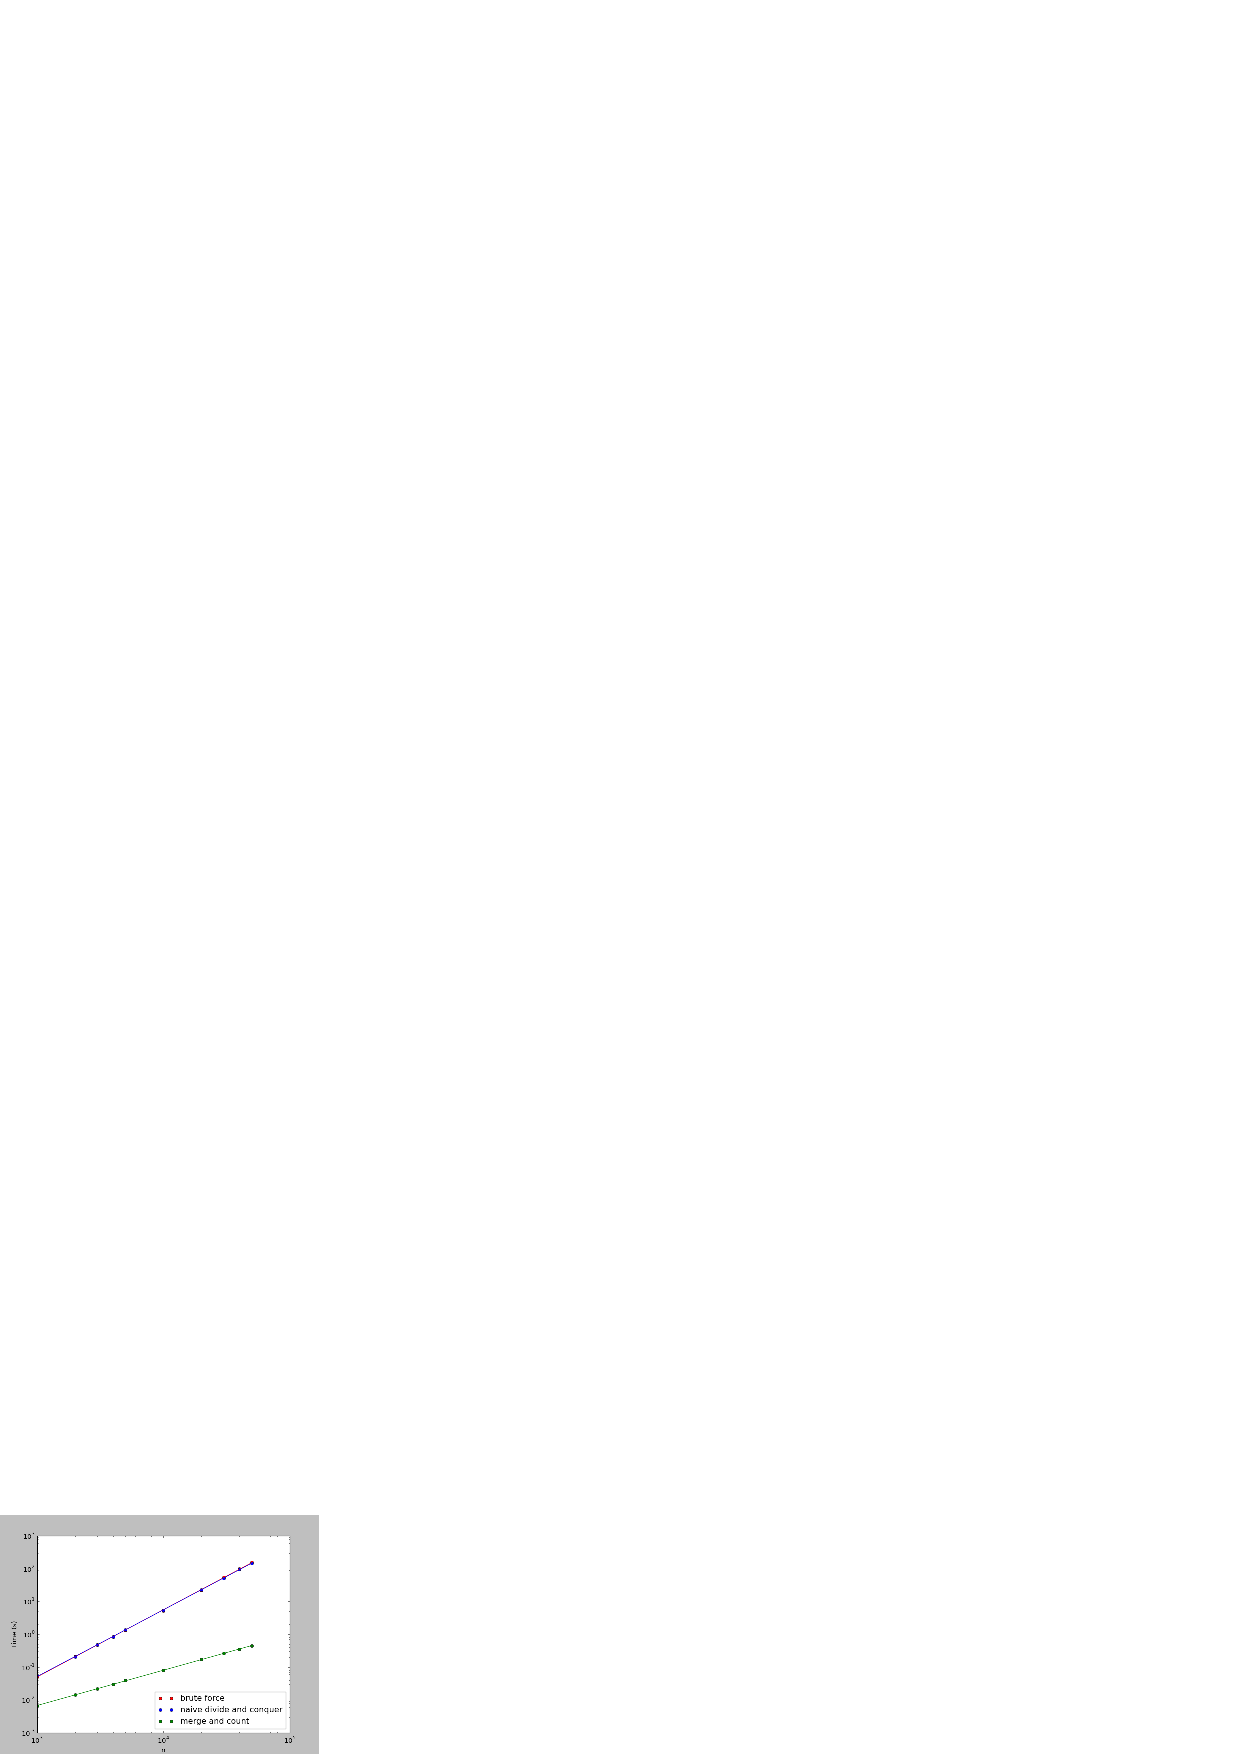
\includegraphics[width=4.5in]{loglog.png}
\end{center}

\newpage

\begin{centering}
\textbf{Slope of lines in log-log plot:}
\end{centering}

The equation for the best fit line on the log-log plot (calculated using numpy.polyfit()) has the following form:

f(n) = e\textsuperscript{y-intercept} * n\textsuperscript{slope}

Brute Force:
\begin{itemize}
\item slope: 2.0177140011
\end{itemize}

Divide \& Conquer:
\begin{itemize}
\item slope: 1.09279503259
\end{itemize}

Dynamic Programming:
\begin{itemize}
\item slope: .996887276493
\end{itemize}

\begin{centering}
\textbf{Performance Comparison}
\end{centering}

Over the range of array sizes under test, Divide and Conquer always performs better than Brute Force, and the Dynamic Programming algorithm always performs better than Divide and Conquer. Sometimes it's necessary to use more temporary memory in order to get performance gains, especially in the case of dynamic programming. But that's not the case here. Some memory usage tests were performed as well, but the results were boring (i.e. no noticeable differences between the algorithms) and don't warrant a graph. 

So in conclusion - for solving the maximum subarray problem, you probably should always use some version of the dynamic programming algorithm presented here.

\end{document}
